\chapter{機械学習を用いた Coincidence Window の作成手法}
本章では機械学習を用いてCWを作成する手法について述べる。
本研究では、シミュレーション用のCWと実際の測定用のCWをそれぞれ作成している。
また、作成したCWの性能について、それぞれ評価を行う。

\section{機械学習を使う方針}
MC Dataを分けて学習\\


\section{本研究で用いる機械学習}
機械学習とは、データからコンピュータが自動で特徴量やルールを学習し、学習した結果に基づいて新たなデータに対し分類や予測を行う分析手法の一つである。
そのため、人がコンピュータにルールを明示的に与える代わりに、学習するためのデータを与えることでコンピュータが自動的にデータからルールを獲得することができるのである。

\subsection{機械学習の学習手法}
機械学習には、教師あり学習、教師なし学習、強化学習といった代表的な学習手法がある。

\subsubsection{教師あり学習}
教師あり学習の目標は、入力$x$から推定したい出力$y$を予測できるようなモデル$y = f(x;\theta)$を学習することである。
教師あり学習では、入力$x$と出力$y$を

\subsubsection{回帰問題}

\subsubsection{分類問題}

\subsection{機械学習モデル}
\subsubsection{パーセプトロン}

\subsubsection{ニューラルネットワーク}
ニューラルネットワークは入力に対し、線形変換と非線形変換を繰り返し適応することで、入力から予測値を計算することができる。
\begin{figure}[tb]
  \centering
  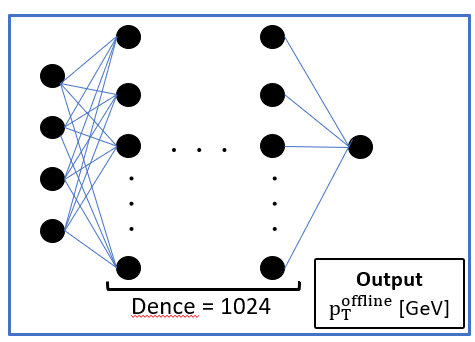
\includegraphics[clip, width=10cm]{fig/4/MLP.png}
  \caption{Resolution}
  \label{fig:Resolution}
\end{figure}


\subsubsection{・活性化関数}

\subsubsection{・損失関数}

\section{機械学習を用いた Coincidence Window の作成}
\subsection{入力データに対する事前処理}
・磁場構造に考慮した領域分け<学習領域の図>\\
\begin{figure}[tb]
  \centering
  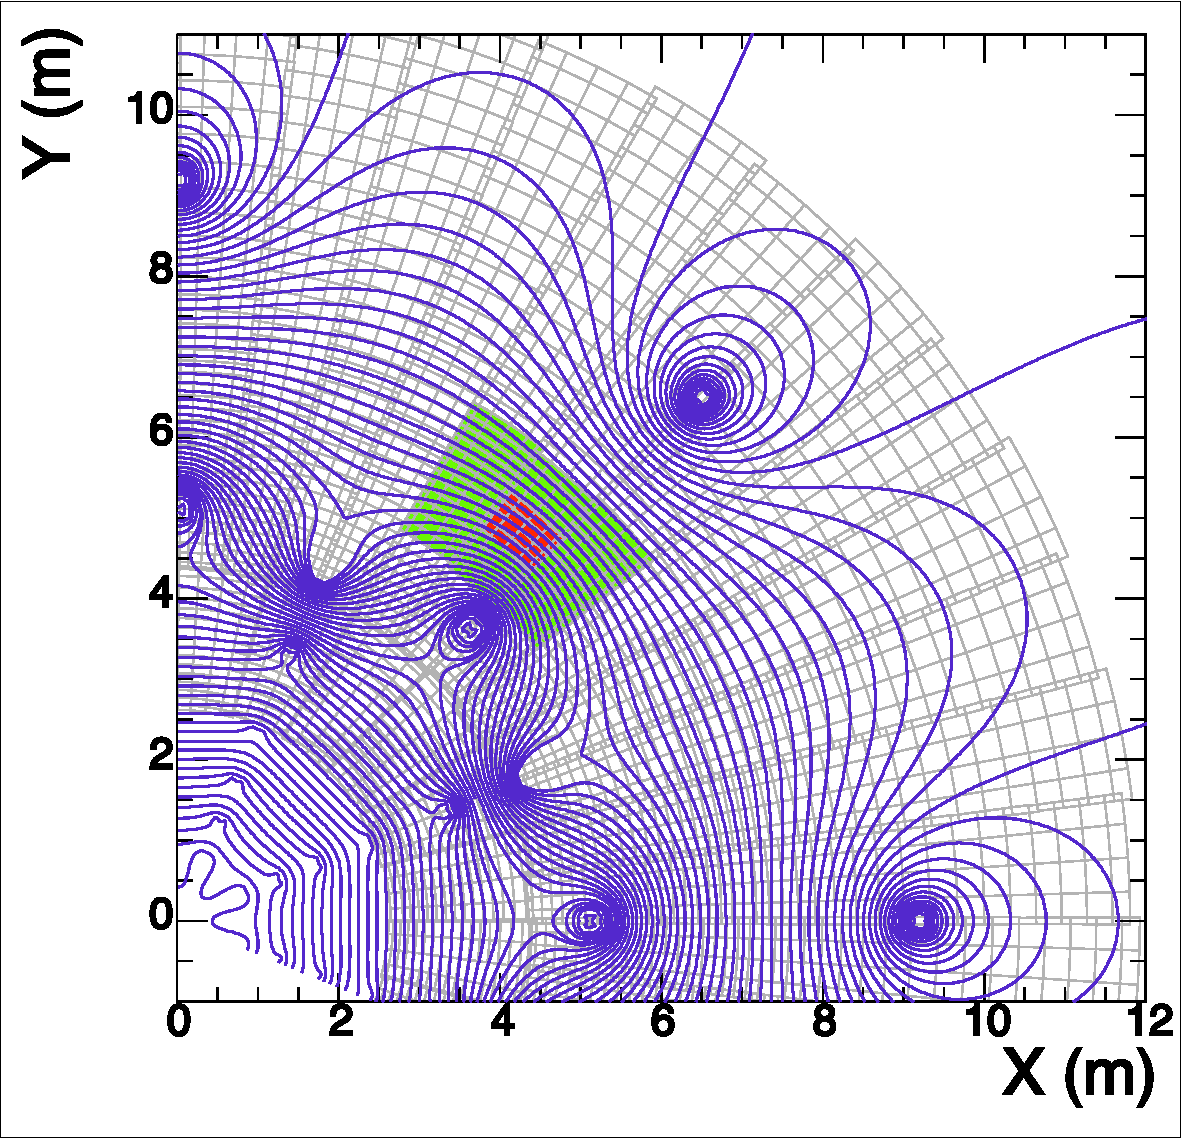
\includegraphics[clip, width=7cm]{fig/4/c1_withMag.pdf}
  \caption{Resolution}
  \label{fig:Resolution}
\end{figure}

・ヒットマップクリーナ<クリーナー前後のhitmap>
\begin{figure}[tb]
  \centering
  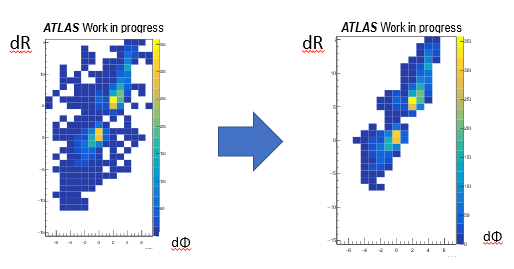
\includegraphics[clip, width=14cm]{fig/4/cleaner.png}
  \caption{Resolution}
  \label{fig:Resolution}
\end{figure}


\subsection{Coincidence Window 作成に向けた機械学習モデルのトレーニング}
・Tensorflow\\
・モデルのトレーニング\\
・パラメータ\\
・機械学習としての性能評価

\subsection{Coincidence Window}
look-up tableの形にする
4bit
fit
出力を閾値に変更

・Efficiencyに対するfitting <fittingの定義のプロット><threshould><Resolution><プラトー>\\
\begin{figure}[tb]
  \centering
  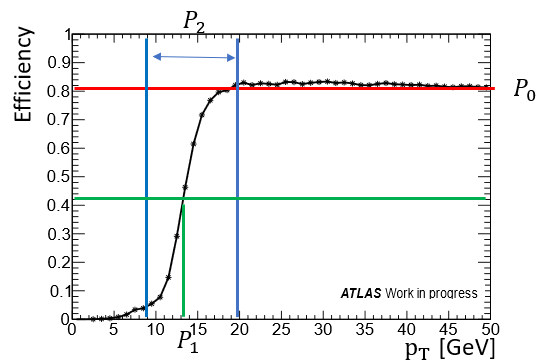
\includegraphics[clip, width=14cm]{fig/4/fitting_def.png}
  \caption{fittingの定義}
  \label{fig:fit_def}
\end{figure}

\begin{figure}[tb]
  \centering
  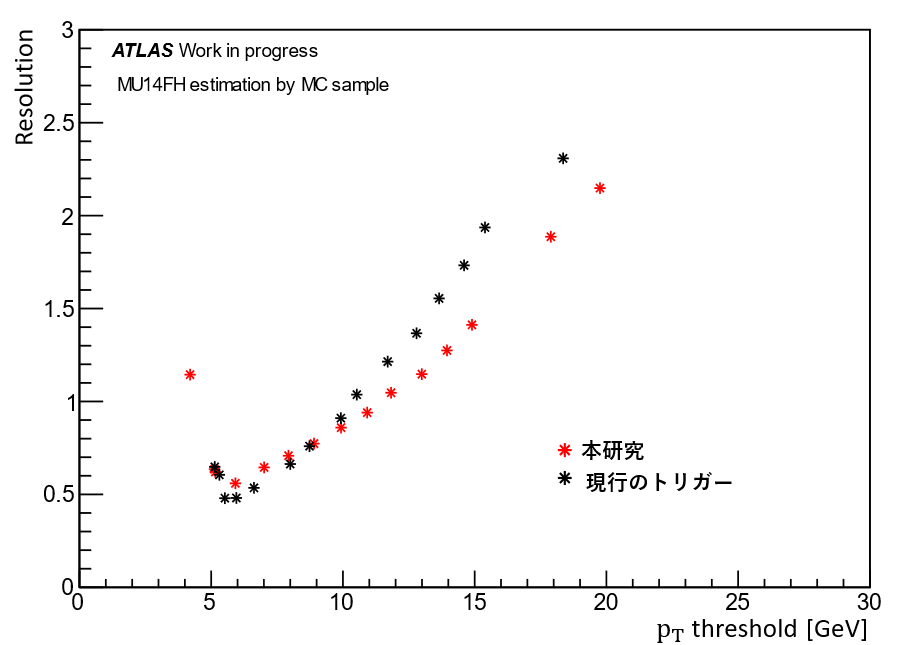
\includegraphics[clip, width=14cm]{fig/4/resolution_v07_v05.png}
  \caption{Resolution}
  \label{fig:Resolution}
\end{figure}



\subsection{Coincidence Window の評価}
Run-2データを用いた評価

<15段階の閾値のEfficiency>
\begin{figure}[tb]
  \centering
  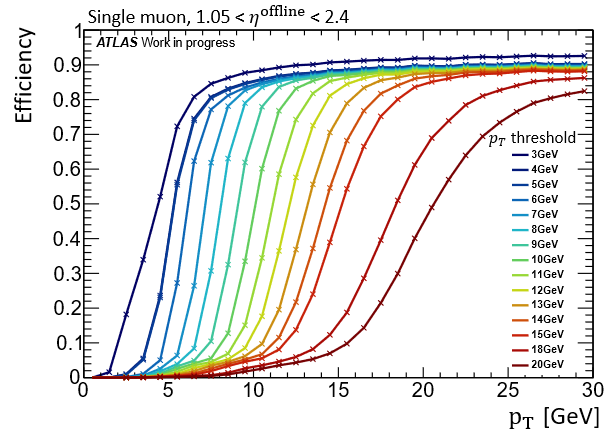
\includegraphics[clip, width=14cm]{fig/4/v07_15_Eff.png}
  \caption{Resolution}
  \label{fig:Resolution}
\end{figure}


<15段階それぞれのEfficiency(v05 vs v06,v07)>\\
\begin{figure}[tb]
  \centering
  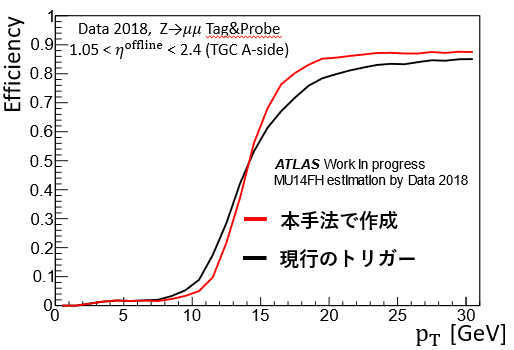
\includegraphics[clip, width=14cm]{fig/4/hikaku_v05_v06.png}
  \caption{v05v06}
  \label{fig:Resolution}
\end{figure}

\begin{figure}[tb]
  \centering
  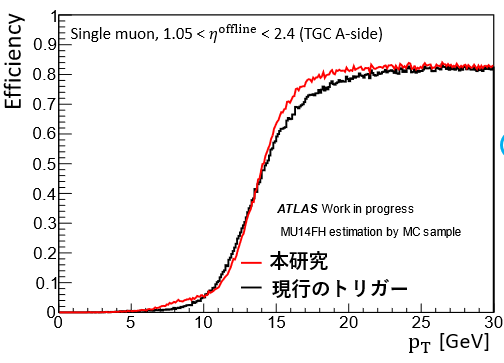
\includegraphics[clip, width=14cm]{fig/4/hikaku_v05_v07.png}
  \caption{v05v07}
  \label{fig:Resolution}
\end{figure}

<MCとDataの比較>
\begin{figure}[tb]
  \centering
  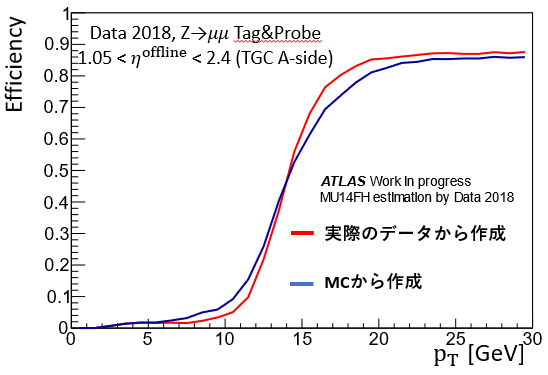
\includegraphics[clip, width=14cm]{fig/4/hikaku_v06_v07.png}
  \caption{v06v07}
  \label{fig:Resolution}
\end{figure}

<TriggerRate>
\begin{figure}[tb]
  \centering
  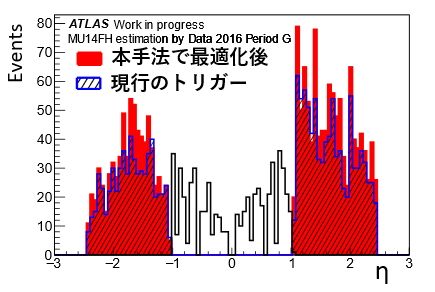
\includegraphics[clip, width=14cm]{fig/4/rate_v05_v06.png}
  \caption{v05v06}
  \label{fig:Resolution}
\end{figure}

